\section*{Łączenie wyjaśnień różnych metod}
W tej sekcji przeanalizowano połączenie wyjaśnień generowanych przez różne matody XAI: LIME, SHAP i GradCAM.
Celem było sprawdzenie, czy łączenie tych metod może dostarczyć bardziej szczegółowych lub ogólnych wyjaśnień.
Przeprowadzimy analizę na całym zbiorze danych, porównując wyniki uzyskane z połączenia wyjaśnień przez część wspólną oraz sumę obszarów

\subsection*{Część wspólna}
W tej analizie połączono wyjaśnienia różnych metod poprzez część wspólną obszarów wyjaśnionych przez każdą z metody.

\begin{figure}[h]
	\centering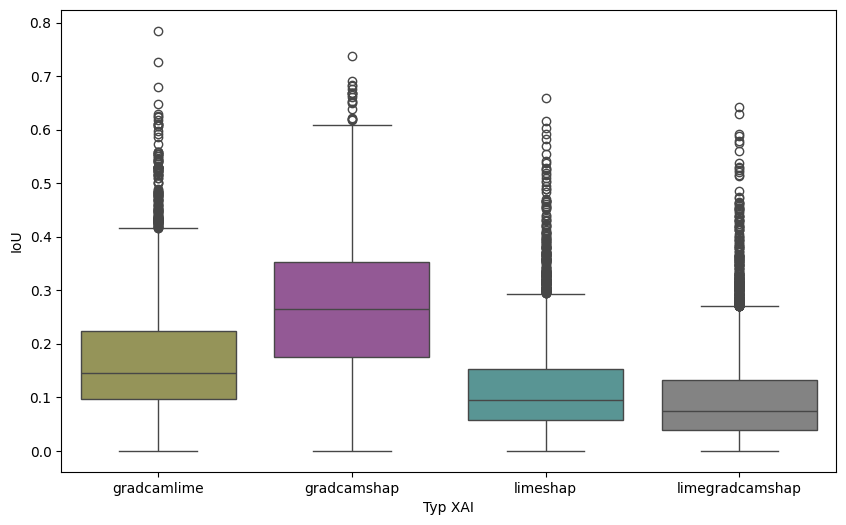
\includegraphics[width=.9\textwidth]{img/combine_iou_and}
	\caption{IoU dla połączeń wyjaśnień poprzez część wspólną}  \label{rys:combine_iou_and}
\end{figure}
\begin{table}[h]
	\centering
	\begin{tabular}{|c|c|}
		\hline
		\textbf{Metoda XAI}  & Średnie IoU \\
		\hline
		GradCAM i LIME       & 0.171258    \\
		\hline
		GradCAM i SHAP       & 0.266315    \\
		\hline
		SHAP i LIME          & 0.117069    \\
		\hline
		GradCAM, LIME i SHAP & 0.099034    \\
		\hline
	\end{tabular}
	\caption{Średnie wartości IoU części wspólnej połączonych wyjaśnień}
	\label{tab:combineandiouand}
\end{table}
Tabela \ref{tab:combineandiouand} średnie wartości dla połączonych wyjaśnień różnych metod XAI.

Najlepsze wyniki osiągnąło połączenie wyjaśnień GradCAM oraz SHAP.
Najgorsze wyniki osiągneło połączenie wszystkich trzechwyjaśnień.
Żadne z połączeń nie uzyskało lepszego średniego wyniku  IoU niż średni wynik którgokolwiek z części wyjaśnień.
Powodem jest zbyt duże zmniejszenie wielkość wyjaśnień.

\begin{figure}[h]
	\centering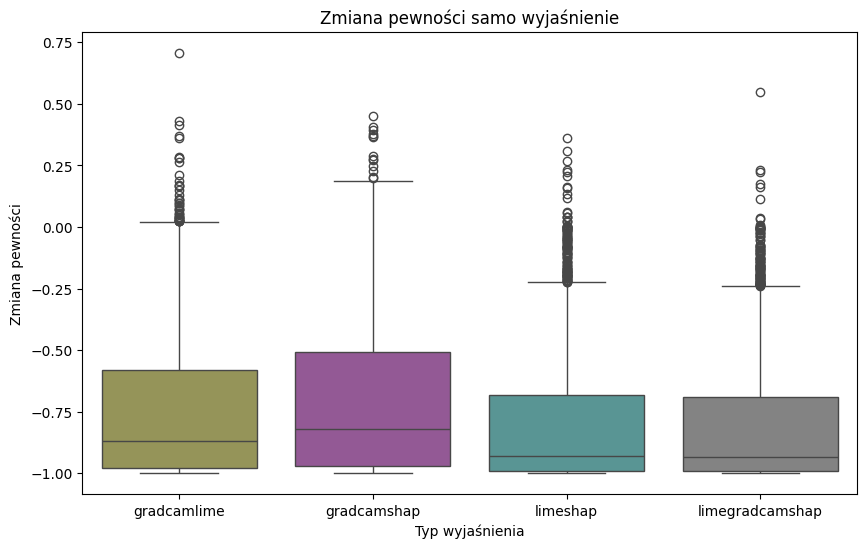
\includegraphics[width=.9\textwidth]{img/combine_confidence_exp_and}
	\caption{Zmiana pewności po pozostawieniu samego wyjaśnienia}  \label{rys:combineandconfidencean}
\end{figure}
\begin{table}[h]
	\centering
	\begin{tabular}{|c|c|}
		\hline
		\textbf{Metoda XAI}  & Zmiana pewności \\
		\hline
		GradCAM i LIME       & -0.748150       \\
		\hline
		GradCAM i SHAP       & -0.702578       \\
		\hline
		SHAP i LIME          & -0.808155       \\
		\hline
		GradCAM, LIME i SHAP & -0.814570       \\
		\hline
	\end{tabular}
	\caption{Średnia zmiana pewności po pozastwieniu sum obszarów samego wyjaśnia}
	\label{tab:combineandconfidenceand}
\end{table}
Zmiana pewności po pozostawieniu samego wyjaśnienia została przedstawiona na \ref{rys:combineandconfidencean} oraz w tabeli \ref{tab:combineandconfidenceand}.
Najlepsze wyniki dla połączenia GradCAM z SHAP, jednak zadal gorsze niż wyjaśnienie uzyskane z samego GradCAM lub samgeo SHAPA.
Żadne z połączeń nie uzyskało lepszego średniego zmiany pewności niż średni wynik którgokolwiek z części wyjaśnień.

\begin{figure}[h]
	\centering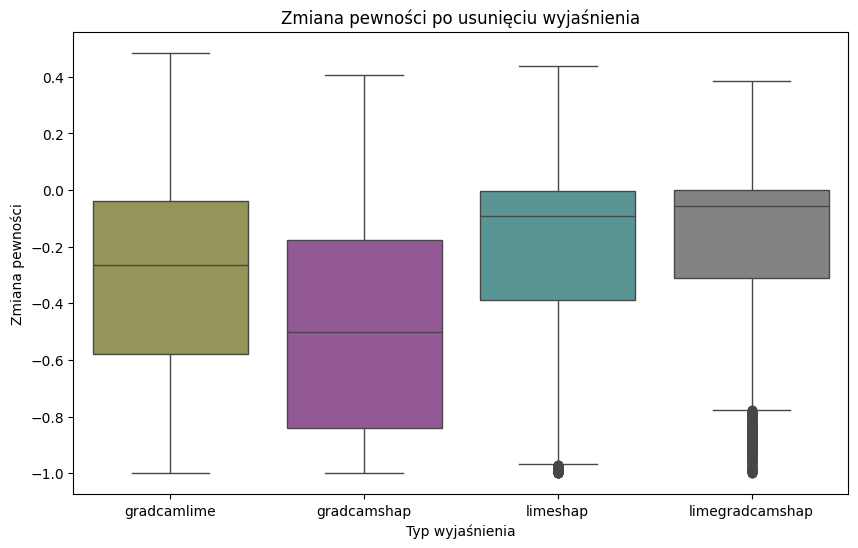
\includegraphics[width=.9\textwidth]{img/combine_confidence_no_exp_and}
	\caption{Zmiana pewności przy usunięciu obszarów wyjaśnienia}  \label{rys:combineandconfidenceandno}
\end{figure}
\begin{table}
	\centering
	\begin{tabular}{|c|c|}
		\hline
		\textbf{Metoda XAI}  & Zmiana pewności \\
		\hline
		GradCAM i LIME       & -0.335106       \\
		\hline
		GradCAM i SHAP       & -0.498530       \\
		\hline
		SHAP i LIME          & -0.219604       \\
		\hline
		GradCAM, LIME i SHAP & -0.188955       \\
		\hline
	\end{tabular}
	\caption{Średnia zmiana pewności usunięciu sum obszarów samego wyjaśnia}
	\label{tab:combineandconfidenceandno}
\end{table}
Zmiana pewności przy usunięciu obszarów wyjaśnienia zostały przedstawiona na rysunku \ref{rys:combineandconfidenceandno} oraz w tabeli \ref{tab:combineandconfidenceandno}
Najlepsze wyniki były dla połączenia GradCAM oraz SHAP, jdenak nadal gorsze niż którekolwiek z części wyjaśnień.
Żadne z połączeń nie uzyskało lepszego średniego zmiany pewności niż średni wynik którgokolwiek z części wyjaśnień.


\subsection*{Suma obszarów}
\begin{figure}[h]
	\centering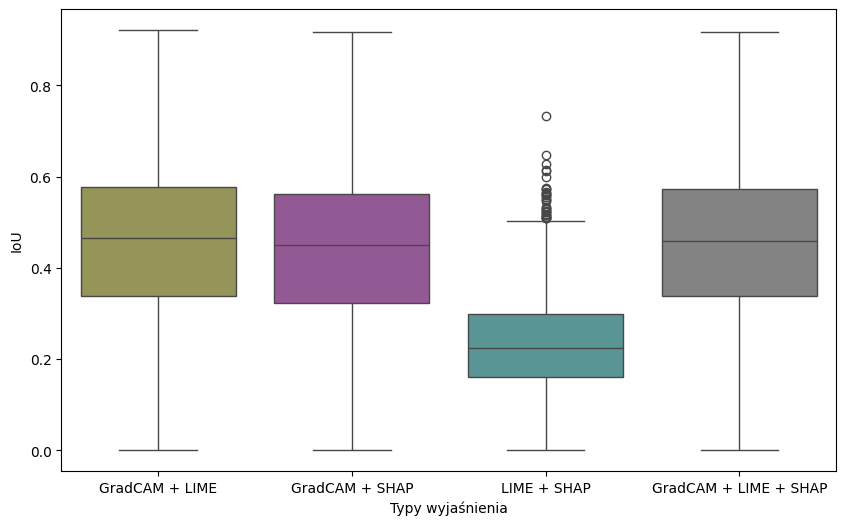
\includegraphics[width=.9\textwidth]{img/combine_iou_or}
	\caption{IoU dla połączeń wyjaśnień poprzez sume obszarów}  \label{rys:combine_iou_or}
\end{figure}
\begin{table}[h]
	\centering
	\begin{tabular}{|c|c|}
		\hline
		\textbf{Metoda XAI}  & Średnie IoU \\
		\hline
		GradCAM i LIME       & 0.454488    \\
		\hline
		GradCAM i SHAP       & 0.419922    \\
		\hline
		SHAP i LIME          & 0.335781    \\
		\hline
		GradCAM, LIME i SHAP & 0.425337    \\
		\hline
	\end{tabular}
	\caption{Średnie wartości IoU części wspólnej połączonych wyjaśnień}
	\label{tab:combineandiou}
\end{table}
Tabela \ref{tab:combineandiou} średnie wartości dla połączonych wyjaśnień różnych metod XAI.
Najlepszy wynik uzsykano z połączenia wyjaśnień GradCAM oraz SHAP.
Dla połączenia wszystkich trzech wyjaśnień wyniki były niższe.
Oznacza to że wyjaśnienia SHAP zawierają obszary będące poza obszarem zainteresowania.
Najgorsze wyniki osiągnął SHAP oraz LIME.
Nadal jednak byłu lepsze niż sam LIME lub sam SHAP.

\begin{figure}[h]
	\centering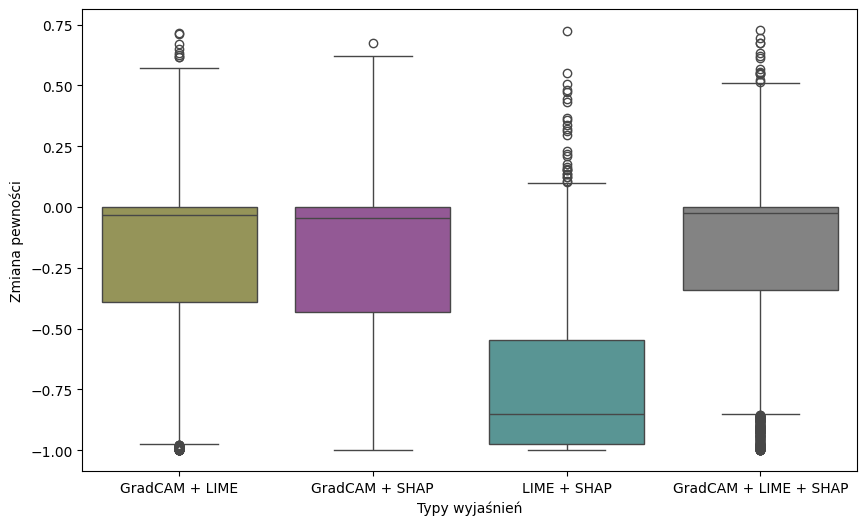
\includegraphics[width=.9\textwidth]{img/combine_confidence_exp_or}
	\caption{Zmiana pewności po pozostawieniu samego wyjaśnienia}  \label{rys:combineandconfidenceor}
\end{figure}
\begin{table}[h]
	\centering
	\begin{tabular}{|c|c|}
		\hline
		\textbf{Metoda XAI}  & Zmiana pewności \\
		\hline
		GradCAM i LIME       & -0.171717       \\
		\hline
		GradCAM i SHAP       & -0.120143       \\
		\hline
		SHAP i LIME          & -0.380949       \\
		\hline
		GradCAM, LIME i SHAP & -0.089013       \\
		\hline
	\end{tabular}
	\caption{Średnia zmiana pewności samych obszarów części wsþlnej połączonych wyjaśnienia}
	\label{tab:combineandconfidenceor}
\end{table}
Zmiana pewności po pozostawieniu samego wyjaśnienia została przedstawiona na \ref{rys:combineandconfidenceor}oraz w tabeli \ref{tab:combineandconfidenceor}.
Najlepszy wynik uzyskało połączenie wszystkich trzech wyjaśnień, co dało znacznie lepsze wyniki niż użycie jedngo wyjaśnienia.
Spowodowane to było mniejszą modeyfikacją.
Najgorsze wyniki uzyskało połączenie SHAP oraz LIME, nadal będąc lepszym wynikiem niż którekolwiek z pojedyńczych części.

\begin{figure}[h]
	\centering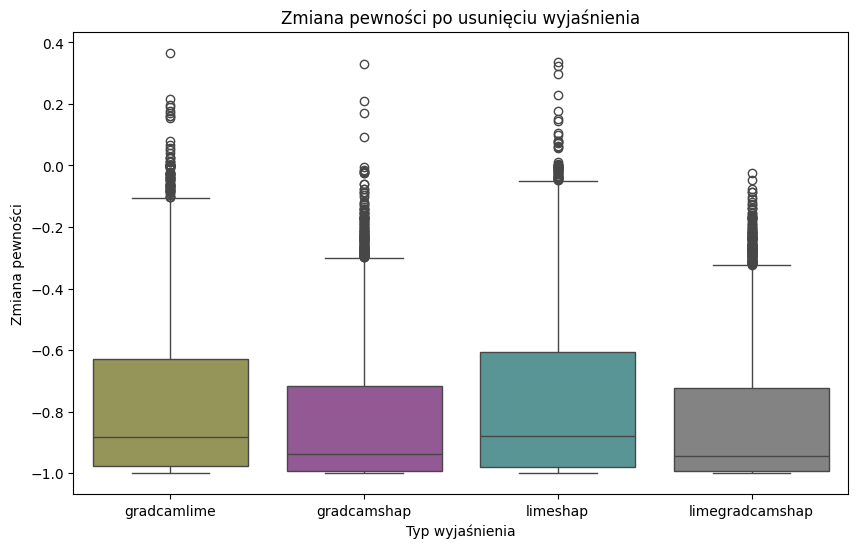
\includegraphics[width=.9\textwidth]{img/combine_confidence_no_exp_or}
	\caption{Zmiana pewności przy usunięciu obszarów wyjaśnienia}  \label{rys:combineandconfidenceorno}
\end{figure}
\begin{table}[h]
	\centering
	\begin{tabular}{|c|c|}
		\hline
		\textbf{Metoda XAI}  & Zmiana pewności \\
		\hline
		GradCAM i LIME       & -0.777072       \\
		\hline
		GradCAM i SHAP       & -0.825787       \\
		\hline
		SHAP i LIME          & -0.771558       \\
		\hline
		GradCAM, LIME i SHAP & -0.832645       \\
		\hline
	\end{tabular}
	\caption{Średnia zmiana pewności usunięciu obszarów}
	\label{tab:combineandconfidenceorno}
\end{table}
Zmiana pewności po pozostawieniu samego wyjaśnienia została przedstawiona na \ref{rys:combineandconfidenceorno}oraz w tabeli \ref{tab:combineandconfidenceorno}.
Najlepszy wynik uzyskało połączenie wszystkich trzech wyjaśnień.
Najgorsze połączenie LIME i SHAP oraz na podobnym poziomie połączenie GradCAM oraz LIME.
Wszystkie przykłady są lepsze niż samo wyjaśnienie.
